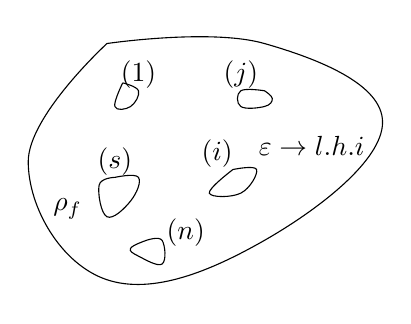
\begin{tikzpicture}

\draw  plot[smooth, tension=.7] coordinates {(-0.5,2.5) (-1.5,1) (-0.5,-0.5) (1.5,0) (3,1.5) (1.5,2.5) (-0.5,2.5)};
\draw  plot[smooth, tension=.7] coordinates {(-0.3,2) (-0.4,1.7) (-0.2,1.7) (-0.1,1.9) (-0.3,2)};
\draw  plot[smooth, tension=.7] coordinates {(1.5,1.9) (1.2,1.9) (1.2,1.7) (1.5,1.7) (1.6,1.8) (1.5,1.9)};
\draw  plot[smooth, tension=.7] coordinates {(1.1,0.9) (0.8,0.6) (1.2,0.6) (1.4,0.9) (1.1,0.9)};
\draw  plot[smooth, tension=.7] coordinates {(-0.4,0.8) (-0.6,0.7) (-0.5,0.3) (-0.2,0.5) (-0.1,0.8) (-0.4,0.8)};
\node at (1.2,2.1) {$(j)$};
\node at (0.9,1.1)  {$(i)$};
\node at (-0.4,1)  {$(s)$};
\node at (0.5,0.1)  {$(n)$};
\draw  plot[smooth, tension=.7] coordinates {(0,0) (-0.2,-0.1) (-0.1,-0.2) (0.2,-0.3) (0.2,0) (0,0)};
\node at (-0.1,2.1) {$(1)$};
\node at (2.1,1.2) {$\varepsilon\rightarrow l.h.i$};
\node at (-1,0.4) {$\rho_f$};
\end{tikzpicture}